\chapter{Representations of Logical Functions}
\label{chapter:Representations of Logical Functions}
\graphicspath{ {./chapter02/Fig} }

A digital system starts its life deep inside an engineer's mind.  
In the beginning it is an abstract device; its very far removed 
from reality.  In order to realize the digital system, the engineer
undertakes the design process; a series of refinements to bring
the digital system closer and closer to a real working system.  This 
iterative approach is necessary in complex designs because going straight
to a final implementation is overwhelming, error-prone, difficult
to modify, and difficult to debug and test.  The goal in breaking the 
design process into steps is to allow the proper specification of the
digital system using a ``language" which is easy to understand and modify,
and then to show how to implement this specification using real circuit 
elements. 

Four refinements in the design of digital systems are 
considered.  Each of these refinements define the input, output, and 
behavior of the digital system.  

\begin{description}
\item [Word Statement] - A written description of the expected 
	input, output, and behavior of the digital system.
\item [Truth Table] -  A listing of every possible input to the
	digital system and the corresponding output.  
\item [Symbolic] - A symbolic (math-like) description of the 
	output(s) as a function of the input variable(s).
\item [Circuit Diagram] - A pictorial representation of the 
	physical interconnections of the circuit elements.
\end{description}

When designing a digital system each of these representations should
describe the same system, just in different ways.  The most abstract 
representation of a digital system is the word statement.  Word 
statements are notoriously ambiguous and have no standardized structure.  
However, these shortcomings are the strengths of this representation. The great
expressibility of language allows very complex processes to be captured 
in brief statements.  Hence, ideas can be quickly refined 
without having to expend much engineering effort.  Also, because 
word statements have no prescribed form, there is a great deal 
of flexibility in structuring a word statements.  Because of its
potential ambiguity and unclear boundaries, the word statement's step 
in the design process diagram shown in Figure~\ref{fig:representationsDesign} is 
drawn inside a puffy cloud.

\begin{figure}[ht]
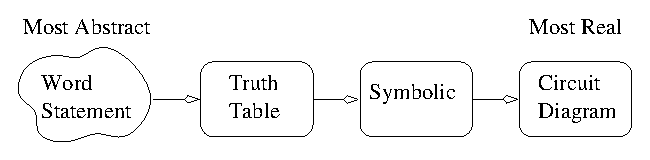
\includegraphics{Design}
\caption{The steps in the design of a digital system.}
\label{fig:representationsDesign}
\end{figure}

Each of the four design stages shown in Figure~\ref{fig:representationsDesign} 
is a description of a digital system.  The arrows in 
Figure~\ref{fig:representationsDesign} are 
transformations described in this chapter.  

After the word statement, all subsequent stages of the design process
are unambiguous, they have one clearly understood interpretation.  The first
refinement of a word statement is a truth table.  The truth table strikingly 
illustrates the difference between digital and analog circuits.  When
working with analog phenomena, like the AC voltage from a wall outlet,
it is impossible to list all possible values of the voltage, because 
an infinite number of potential values exists.  However, when working
with digital phenomena, each signal can have only one of two possible values,
making it quite easy to enumerate them all.  When working with a
digital system with three bits of inputs, like that shown in 
Figure~\ref{fig:numberingSys}, there are only eight
different combinations of the inputs.  For each of these input 
combinations, a truth table specifies what the output should be.  

The symbolic form is a set of equations written in Boolean Algebra.
These equations look similar to those encountered
in an algebra class. However, instead of operations like addition 
and multiplication, Boolean Algebra uses the operations AND, OR, and 
NOT.  These operations have hardware counterparts - real physical 
circuits which ``compute" their values.  A circuit diagram shows how
these hardware components are interconnected to realize the 
digital system.  As real devices, these circuits represent the bit 
values, 0 and 1 as voltages.  Typically, logic 1 is represented by 
a high voltage level (5v) and logic 0 is represented by a low 
voltage level (0v). 

This text takes a bottom-up approach in designing digital systems.  
The design process starts with the most fundamental digital hardware 
components and shows how they are interconnected to form basic building 
blocks.  These building blocks are then arranged into datapath and 
control circuit.  Thus, all the digital circuits studies in this text
will be built from a small pallet of fundamental digital hardware 
components, called the elementary logical functions.

\section{Elementary Logical Functions}
\label{section:representationsElementaryLogicalFunction}
Elementary logical functions get their name because they are 
the fundamental (elementary) building blocks of digital design, they 
use the logical operators like AND, OR, and NOT (logical), and 
they describe a transformation (function) from input to output.  For each 
elementary logical function, its word statement, truth table, symbolic and 
circuit diagram are presented.


\label{page:elf1}
\begin{tabular}{ll}

{\huge AND} & 
\begin{tabular}{l|l}
Word Statement &  
\begin{tabular}{l}
AND is a logical function with two inputs and   \\
one output.  The output equals 1 only when all the \\
inputs are equal to 1, otherwise the output   \\
equals 0. 
\end{tabular} \\ \hline
Symbolic  & A*B \\ \hline
Truth Table &
	\begin{tabular}{c|c||c}
	A & B & A*B \\ \hline \hline
	0 & 0 & 0   \\ \hline
	0 & 1 & 0   \\ \hline
	1 & 0 & 0   \\ \hline
	1 & 1 & 1   \\ 
	\end{tabular} \\ \hline
Circuit Diagram & 
\includegraphics{and} \\
%% \end{tabular} \\ \hline \hline
\end{tabular} \\ 
\end{tabular}

\begin{tabular}{ll}
{\huge OR} &
\begin{tabular}{l|l}
Word Statement &
\begin{tabular}{l}
OR is a logical function with two inputs and one  \\
output.  The output equals 1 when any input  \\
is equal to 1, otherwise the output equals 0. \\
\end{tabular} \\ \hline
Symbolic &  A+B \\ \hline
Truth Table &
	\begin{tabular}{c|c||c}
	A & B & A+B \\ \hline \hline
	0 & 0 & 0   \\ \hline
	0 & 1 & 1   \\ \hline
	1 & 0 & 1   \\ \hline
	1 & 1 & 1   \\ 
	\end{tabular} \\ \hline
Circuit Diagram & 
\includegraphics{or} \\
\end{tabular} \\ \hline \hline

{\huge NOT} & 
\begin{tabular}{l|l}
Word Statement &
\begin{tabular}{l}
NOT is a logical function with one input and one  \\
output.  The output is not equal to the input. \\
\end{tabular} \\ \hline
Symbolic & A' \\ \hline
Truth Table &
	\begin{tabular}{c||c}
	A & A' \\ \hline \hline
	0 & 1   \\ \hline
	1 & 0   \\ 
	\end{tabular} \\ \hline
Circuit Diagram & 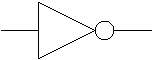
\includegraphics{not} \\
\end{tabular} \\ \hline \hline

{\huge NAND} & 
\begin{tabular}{l|l}
Word Statement &
\begin{tabular}{l}
NAND is a logical function with two inputs and \\
one output.  The output equals 1 when any input \\
is equal to 0, otherwise the output equals 0. \\
\end{tabular} \\ \hline
Symbolic &  (A*B)' \\ \hline
Truth Table & 
	\begin{tabular}{c|c||c}
	A & B & (A*B)' \\ \hline \hline
	0 & 0 & 1   \\ \hline
	0 & 1 & 1   \\ \hline
	1 & 0 & 1   \\ \hline
	1 & 1 & 0   \\
	\end{tabular} \\ \hline
Circuit Diagram & 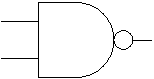
\includegraphics{nand} \\
\end{tabular} \\ \hline \hline
\end{tabular}

\begin{tabular}{ll}
{\huge NOR} & 
\begin{tabular}{l|l}
Word Statement & 
\begin{tabular}{l}
NOR is a logical function with two inputs and  \\
one output.  The output equals 0 when any input  \\
is equal to 1, otherwise the output equals 0. \\
\end{tabular} \\ \hline
Symbolic & (A+B)' \\ \hline
Truth Table &
	\begin{tabular}{c|c||c}
	A & B & (A+B)' \\ \hline \hline
	0 & 0 & 1   \\ \hline
	0 & 1 & 0   \\ \hline
	1 & 0 & 0   \\ \hline
	1 & 1 & 0   \\
	\end{tabular} \\ \hline
Circuit Diagram & 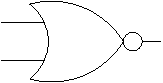
\includegraphics{nor} \\
\end{tabular} \\ \hline \hline

{\huge XOR} & 
\begin{tabular}{l|l}
Word Statement &
\begin{tabular}{l}
XOR is a logical function with two inputs and  \\
one output.  The output equals 1 when the inputs  \\
are different, otherwise the output is equal  \\
to 0.
\end{tabular} \\ \hline
Symbolic & $A \oplus B$ \\ \hline
Truth Table &
	\begin{tabular}{c|c|c}
	A & B & A $\oplus$ B \\ \hline \hline
	0 & 0 & 0   \\ \hline
	0 & 1 & 1   \\ \hline
	1 & 0 & 1   \\ \hline
	1 & 1 & 0   \\ 
	\end{tabular} \\ \hline
Circuit Diagram & 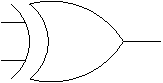
\includegraphics{xor} \\
\end{tabular} \\ \hline \hline
%% \caption{The elementary logical functions.}
%% \label{table:elf}
\end{tabular}
\label{page:elf2}

The physical elements for the elementary logical functions are
typically called \textit{gates}.   Thus, the physical circuit for 
the AND logical function is called an AND gate.

The AND/OR functions can be enlarged to handle more than
two inputs because their word statements use words ALL/ANY
respectively.  Thus a 4-input AND gate will output 1
only when all four inputs equal 1.  The circuit diagram for 
this AND gate would look just like a 2-input AND gate with
two additional inputs.

\section{Conversion Between Representations}
Figure~\ref{fig:representationsForms} shows the four representations of a digital system
along with the different transformations covered in this section.  
The arrows are numbered by the subsection in which the transformation is
covered.  The design process shown in Figure~\ref{fig:Design} is captured
in Steps 7, 6, and 3.  The other transformations introduced in this 
section enable designs to be optimized as well as to explore 
the relationships between the representations.

\begin{figure}[ht]
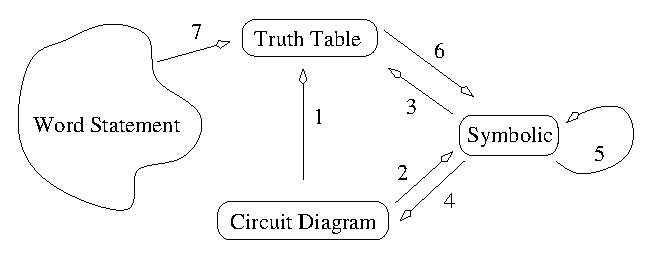
\includegraphics{forms}
\caption{The four representations of a logical function.  The
numbered arrows are the transformations examined in this chapter.}
\label{fig:representationsForms}
\end{figure}

\subsection{Circuit Diagram to Truth Table}

The first transformation is the circuit diagram to truth table.  
Where the circuit diagram came from is unimportant for now.
Figure~\ref{fig:representationsCD-TT} is a circuit diagram with three bits of 
input labeled $A,B,C$ and one bit of output $F(A,B,C)$ that will
be transformed into a truth table.

\begin{figure}[ht]
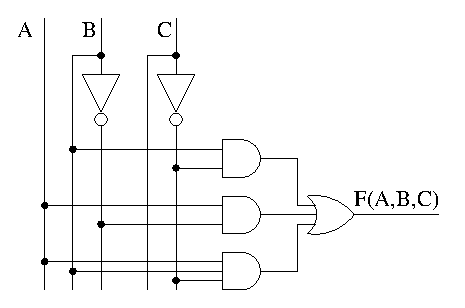
\includegraphics{cd-tt}
\caption{A simple 3-input, 1-output circuit.}
\label{fig:representationsCD-TT}
\end{figure}

Before starting with the transformation there are some important
observations to make about Figure~\ref{fig:representationsCD-TT}. 
\begin{enumerate}
\item The gates in a circuit  may have different numbers of inputs.  For example, this circuit contains 
two AND gates with two bits of input and an AND gate with three bits of
input.  
\item The lines drawn in the figure represent physical wire.
\item When a voltage is applied to one end of the wire by an external source
or by one of the gates, it is assumed to propagate instantaneously to 
all points on the wire.  
\item The black dots on intersecting wires means  that the two wires are 
connected.  For example, the vertical wire
labeled ``$A$" is connected to the second and third AND gates. 
\item Wires that cross one another and do not have a dot are assumed not
to be connected.  For example, the $C$ signal does not go into the
second AND gates.  
\item Outputs are never connected directly together, because 
they could create a short-circuit destroying the participating gates.  
\item  Inputs are always tied to some signal source, usually the
output of a gate.
\item A gate output may drive the inputs of many different gates.
\end{enumerate}

Since
the three external inputs in Figure~\ref{fig:representationsCD-TT} do not have sources shown,
they must be provided by some external user.  The output 
from a gate can provide input to multiple, different inputs.  For example, 
the output of the NOT gate
associated with the $C$ input feeds the first and third AND gates. 


\begin{example}{Circuit Diagram to Truth Table}
\label{example:representationCDtoTT}

\emph{\textbf{\ul{Problem:}}}
Convert the circuit diagram in Figure~\ref{fig:representationsCD-TT}
into a truth table.

\noindent\emph{\textbf{\ul{Solution:}}} 

\textbf{Step 1:} Identify the inputs and outputs of the circuit.
Any wire which is not being driven by some source is an input and 
any output which is not driving a source is an output.  In the case of 
Figure~\ref{fig:representationsCD-TT}, $A,B,C$ are inputs and $F(A,B,C)$ is an output.


\textbf{Step 2:} Build the shell of the truth table to hold the solution.  
Remember that, ``A truth table is a listing of every possible  input to the 
digital system and the corresponding output."  For example $A=1$, $B=0$ and 
$C=1$ is a possible input to the circuit.  All the 
potential inputs to the circuit could be listed in a \textit{ad-hoc} 
manner, but a much more organized approach is shown below.

\label{page:TTshell}
$$\begin{array}{c|c|c||c}
A & B & C & F(A,B,C) \\ \hline \hline
0 & 0 & 0 &   \\ \hline
0 & 0 & 1 &   \\ \hline
0 & 1 & 0 &   \\ \hline
0 & 1 & 1 &   \\ \hline
1 & 0 & 0 &   \\ \hline
1 & 0 & 1 &   \\ \hline
1 & 1 & 0 &   \\ \hline
1 & 1 & 1 &   \\
\end{array}$$

Two good reasons drive this choice of row ordering.
First, the columns of the truth table have a strong pattern.
The bits of the $C$-variable column repeat from top to bottom, $0 1 0 1 \ldots$.
The bits of the $B$-variable column repeat from top to bottom, two 0s followed by two 1s.
The bits of the $A$-variable column repeat from top to bottom, four 0s followed by four 1s.
Using this pattern makes filling a truth table easier.  Second,
when the $A,B,C$ variables in each row are interpreted as a 
3-bit binary number, they form consecutive integers.  This approach
makes finding a particular input/output much easier.

\textbf{Step 3:} Determine the values in the $F(A,B,C)$ column.  
In order to do this each input is applied, one at a time, to 
the circuit and determine the output of the circuit.  This step is also
referred to as evaluating the output of the circuit.  

Imagine that 
the bits are flowing down hill from the inputs to the outputs.  A 
gate computes its output only when the values of all its inputs
are known.  The output of a gate is determined from the truth tables
given on pages \pageref{page:elf1} through \pageref{page:elf2}.  For example,
in Figure~\ref{fig:representationsCd-tt2}A, the input $A=B=C=0$ is applied
to the input.  The third AND gate cannot compute its output until
it receives the output from the NOT gate associated with the $C$ 
input.  The outputs from each gate are shown on the signals in
Figure~\ref{fig:figrepresentationsCd-tt2}B.  Due to size constraints, the AND gate 
inputs are written inside the gate.  

%\begin{figure}[ht]
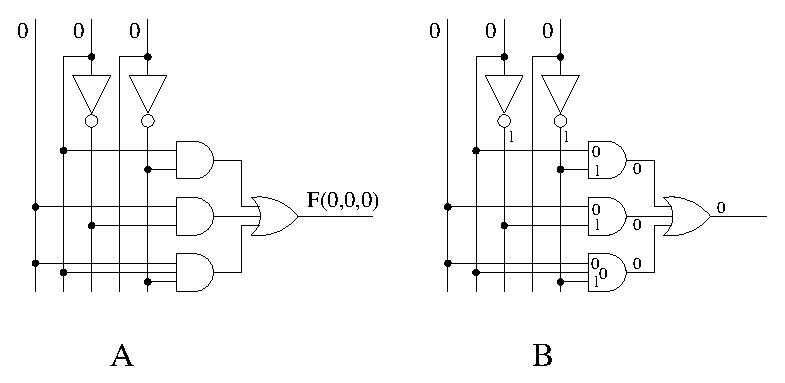
\includegraphics{cd-tt2}
\fakefigure{fig:representationsCd-tt2}

\textbf{Figure:}~\ref{fig:representationsCd-tt2} A) The circuit diagram from Figure~\ref{fig:representationsCD-TT} with input $A=B=C=0$.  B) The effect of this input shown on the wires.
%\end{figure}

Figures \ref{fig:representationsCD-TT} and \ref{fig:representationsCd-tt2} 
illustrate a subtle notational convention. 
Why is the output of the circuit shown in Figure~\ref{fig:representationsCD-TT} 
labeled $F(A,B,C)$ and in Figure~\ref{fig:representationsCd-tt2}A this same output is
labeled  $F(0,0,0)$?  It is because the variables $A,B,C$ in $F(A,B,C)$ 
are placeholders for the actual values of the variables.  Since these
variables are given the values $A,B,C = 0,0,0$ in Figure~\ref{fig:representationsCd-tt2}A, 
this notational change is acknowledged by labeling the output $F(0,0,0)$.

Since Figure~\ref{fig:representationsCd-tt2}B shows that $F(0,0,0) = 0$, then
a 0 is placed in the top row of the truth table for this 
function.  The remaining seven rows of the truth table are computed 
using this same method.  The resulting truth table is shown below.

$$\begin{array}{c|c|c||c}
A & B & C & F(A,B,C) \\ \hline \hline
0 & 0 & 0 & 0  \\ \hline
0 & 0 & 1 & 0  \\ \hline
0 & 1 & 0 & 1  \\ \hline
0 & 1 & 1 & 0  \\ \hline
1 & 0 & 0 & 1  \\ \hline
1 & 0 & 1 & 1  \\ \hline
1 & 1 & 0 & 1  \\ \hline
1 & 1 & 1 & 0  \\
\end{array}$$
\end{example}

While this transformation provides an excellent introduction to a variety
of important concepts, it is not a practical way to derive the truth table 
entries.  First, it is tedious because the same process must be performed 
eight times.  Second, it is prone to errors because the bits on the figure
must be overwritten seven times, once for every row of the table. 
It turns out that determining the symbolic
form for this circuit's output and then determining the truth table is a
much less tedious and less error-prone method to determine the truth table
from a circuit diagram.

\subsection{Circuit Diagram to Symbolic}
The transformation of a circuit diagram into a symbolic expression 
is very similar to evaluating the output of the circuit, except symbols
instead of bits flow through the circuit.  The symbolic output of 
a gate is written out only when symbolic inputs are present on all of the 
gate's input.  The output of a gate is determined from the symbolic forms
given on pages \pageref{page:elf1} and \pageref{page:elf2}.  For example, in 
order to determine the output of the AND gates in Figure~\ref{fig:representationsBasic}A, the
symbolic outputs of the NOT gates must first be determined.  These are
$A', B', C'$ as shown in Figure~\ref{fig:representationsBasic}B.

\begin{figure}[ht]
%% scalebox{0.5}{stuff}
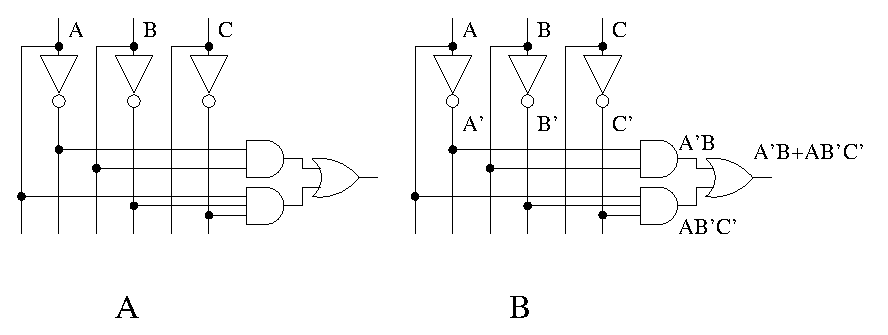
\includegraphics{basic}
\caption{A) A circuit diagram.  B) The input variables propagated through
to the output.}
\label{fig:representationsBasic}
\end{figure}

Since the inputs to the top AND gate are $A'$ and $B$, the output of the AND
gate is labeled $A'B$.  The output was not labeled ``A'*B" because the
``*" is often dropped from the symbolic expressions involving AND 
in order to save space.  This is similar to the convention 
of dropping the ``*" symbol when it is used
as the multiplication operator in regular algebra.  When two Boolean 
variables appear next to one another it is assumed that they are ANDed together.
After labeling the output of the other AND gate, the output of the OR gate 
is labeled $A'B + AB'C'$ as shown in Figure~\ref{fig:representationsBasic}B.

It was earlier suggested that in order to determine the truth table for a
circuit diagram, it is easier to first determine the symbolic form for
the circuit diagram, and then determine the truth table from this symbolic 
form.  Determining the symbolic form of a circuit's output is eight times
easier than determining all eight rows of the truth table.
The next subsection will show how to transform a symbolic 
form into a truth table.

\subsection{Symbolic to Truth Table}

Like the transformation of a circuit diagram to a truth table, the
first step in this transformation is to identify the inputs and outputs 
of the circuit.  Normally, the variable on the left-hand side
of the equal sign in an equation is the output and any variables 
which appear on the 
right-hand side are inputs.  For example, in the equation 
$F(A,B,C) = A'B + AB'C'$, $F$ is the output and $A,B,C$ are the inputs.

The second step is to write down the shell of the truth table using the
ordering given on page~\pageref{page:TTshell}.  The basic structure of the
truth table is the same no matter how many variables the symbolic 
expression has.  
For example, if a symbolic expression has four input variables $A,B,C,D$,
then start by listing the variables across the top of the truth table.  
Then write the bit values for the $D$ variable by alternating 0
and 1 on every row, from top to bottom. The $C$ variable would alternate 
every other row, from top to bottom.  The $B$ variable every
fourth row, and the $A$ variable every eighth row.  The resulting 
truth table has 16 rows.  This should not come as a surprise since,
from page~\pageref{page:two-to-N}, there are 
$2^4=16$ different combinations of four input bits.

The third step in the transformation is to evaluate the symbolic 
expression for each combination of inputs.  Evaluation is the process
of substituting each variable's value into the equation and applying 
the operators to the values.  For example, evaluate $F(A,B) = (A+B)'$
for $(A,B) = (0,1)$.  Substituting in the values for the variables
yields $F(0,1) = (0+1)'$.  Applying the OR operation to 0 and 1 gives the 
result 1.  Applying the NOT operator to the result of the OR operator yields 0.
Thus, $F(A,B)$ evaluated at $(A,B)=(0,1)$ equals 0.  In other words,
$F(0,1)=0$.  The evaluation of more complex expressions requires 
a firm grasp on the rules of operator precedence in Boolean Algebra.

The symbolic expressions are written in 
\textit{Boolean Algebra}, \index{Boolean Algebra} an algebra where variables
represent the values 0 and 1 and which are joined together using operators 
like AND, OR and NOT.  The symbolic expressions written in a 
high school algebra class have variables which represent real numbers and
are joined together using operators like addition and multiplication.  In 
both algebras, operator precedence must be understood in order to evaluate
complex expressions.  Operator precedence specifies the order in which the
operations of an expression are evaluated.  Operations with higher precedence
are performed before operations with lower precedence.  The rules of operator 
precedence are listed for both algebras in the following table.

\begin{tabular}[ht]{l|l|l}
			& Regular Algebra			& Boolean Algebra \\ \hline \hline
High precedence	& Parenthesis			& Parenthesis	\\ \hline
			& Exponents				& Not			\\ \hline
			& Multiplication/Division	& And			\\ \hline
Low precedence	& Addition/Subtraction 		& Or 			\\
\end{tabular}
\\ \\
Operator precedence is examined by considering the problem of
deriving the truth table for the $F(A,B,C) = A'B + AB'C'$.  This expression
has three input variables and one output variable.  An empty shell of the 
truth table is exactly the same as the one shown on 
page~\pageref{page:TTshell}.  

Next, the expression is evaluated for every possible input.  In 
other words, determine $F(0,0,0) \ldots F(1,1,1)$.  Start with 
the first row of the truth table and determine $F(0,0,0)$ by
substituting $0,0,0$ for every occurrence of $A,B,C$ in the symbolic 
expression.  This yields $0'*0+0*0'*0'$.  In order to evaluate this expression, 
perform the highest precedence operator first.  In this case, evaluate 
the three NOTs yielding, $1*0+0*1*1$.  The next highest 
precedence operator is AND, evaluating the two ANDs in the expression 
yields, $0+0$.   Evaluating the remaining OR yields 0.  Hence, $F(0,0,0)=0$.

Continuing this procedure of evaluating the function for the remaining seven
inputs, would result in the same problems encountered when converting  a
circuit diagram into a truth table namely, that the
process is tedious and error prone.  In order to make good on the 
promise to produce an efficient transformation of a circuit diagram 
to a truth table, a better method is needed to complete the truth table
from the symbolic form.

Two conditions make evaluating a symbolic expression
difficult: its size and the evaluation process itself.  Each difficulty
will be addressed in turn.  Instead of treating the symbolic expression 
as a single monolithic entity, break the expression into smaller
subexpressions, evaluate each subexpression for all the inputs, and 
then put the values of the subexpressions back together.  Three criteria govern
the decomposition of an expression into subexpressions. First, break the 
the expression into as few pieces as possible.  Second, break the expression 
into subexpressions which are easy to put back together.  Third, break the
expression into subexpressions which are easy to evaluate.  

For example, look at the expression $A'B + AB'C'$.  This expression splits nicely
into two subexpressions $A'B$ and  $AB'C'$.  This division meets the three
criteria, only two subexpressions are defined, the subexpressions can be put
back together by ORing them, and, as shown next, there is a simple 
way to evaluate the two subexpression.

In order to efficiently evaluate an expression for all of the rows of a 
truth table the number of questions asked about the expression must
be reduced.  This can be done for product terms.
A \textit{product term} \index{product term} is a group of variables 
(or variables negated) which are ANDed together.   For example, $A'B$ and  
$AB'C'$ are both product terms.  Instead of evaluating a product term for each
row of a truth table, ask, ``what input(s) cause the product term to 
evaluate to 1?"  Since AND evaluates to 1 when all its inputs are 1, 
identify the rows of the truth table where the inputs equal 1.
For example the product term $AB'C'$ evaluates to 1 only when $A=1$, $B=0$, and 
$C=0$.  Note, the B and C variables are negated in the product term so the 
variable must equal 0, so that its negation equals 1 before being ANDed.  
On the row $(A,B,C) = (1,0,0)$ the product term $AB'C'$ equals 1.  What
does the product term equal for all the other rows of the truth table?  
Since the product term does not equal 1 for these rows, the only alternative
is for it to equal 0.  Consequently, the remaining seven rows of the truth 
table equal 0 as shown in Table~\ref{table:SymToTT}.

\begin{table}
$$\begin{array}{c|c|c||c|c||c}
A & B & C & A'B & AB'C' & F(A,B,C) \\ \hline \hline
0 & 0 & 0 & 0  &  0 &  0  \\ \hline
0 & 0 & 1 & 0  &  0 &  0  \\ \hline
0 & 1 & 0 & 1  &  0 &  1  \\ \hline
0 & 1 & 1 & 1  &  0 &  1  \\ \hline
1 & 0 & 0 & 0  &  1 &  1  \\ \hline
1 & 0 & 1 & 0  &  0 &  0  \\ \hline
1 & 1 & 0 & 0  &  0 &  0  \\ \hline
1 & 1 & 1 & 0  &  0 &  0 
\end{array} $$
\caption{The truth table for $F(A,B,C) = A'B + AB'C'$ and its 
two subexpressions.}
\label{table:SymToTT}
\end{table}

What inputs cause the product term $A'B$ to equal 1?  Clearly, $A=0$ and $B=1$.
While filling out the truth table for this product term there may be some
confusion
how to handle the $C$ variable.  Since the $C$ variable is not present in the 
product term then its value is irrelevant. Consequently, the product term $A'B$
evaluates to 1 for $(A,B,C)=(0,1,0)$ and $(A,B,C)=(0,1,1)$, and evaluates to 0
for all other inputs as shown in Table~\ref{table:SymToTT}.

Finally, combine these two subexpressions and compute the value
of the function $F(A,B,C) = A'B + AB'C'$ for all rows of the truth table. In 
order to do this, look at each row of the truth table and ORing the value of 
the two
subexpressions together.  Since OR evaluates to 1 when any of its inputs equals
1, then it suffices to look for rows where either of the two subexpressions equal
1 and put a 1 for the output for $F$.  All other rows will equal 0.  The result 
is shown in Table~\ref{table:SymToTT}.

The words \textit{ realize} and \textit{implement} \index{realize} \index{implement} 
are used somewhat interchangeably to mean executing the design
process in order to build a circuit -- to make the digital system real.  
Since this text focuses on the logical 
behavior of circuits, not their physical behavior, the design process ends with
a circuit diagram, see Figure~\ref{fig:Design}.  In general, when asked
to realize or implement a circuit make it as real as 
possible.  Along similar lines, the realization or implementation of a circuit 
is its physical manifestation.  In order to answer questions about a 
digital systems realization or implementation, reason about the behavior of its 
physical implementation.  In the next section the last step in the realization
of of digital systems, symbolic to circuit diagram, is examined.


\subsection{Symbolic to Circuit Diagram}

The transformation of a symbolic expression into a circuit diagram is a journey
from the output of the circuit towards the input.  When a symbolic expression
is evaluated, some operation is always performed last, yielding
the single-bit output of the function.  This operation is the lowest 
precedence operator of the expression because all the higher precedence 
operations have already been performed.  This lowest precedence operator
is the gate which generates the output of the circuit diagram.  Draw this gate
and label its output with the name of the function.  

Now, remove this lowest precedence operator from the parent symbolic 
expression.  This change may create one 
or more child subexpressions, each of which contributes an input to the 
parent gate.  Now, look at each of these child subexpressions, and in turn and 
parse them in the same way the parent process was parsed.  The parsing is a 
4-step process.

\begin{enumerate}
\item Identify the lowest precedence operator in the subexpression,
\item Draw the gate of this lowest precedence operator,
\item Connect this gate's output to an input of its parent gate, and
\item Remove the operation from the subexpression creating one or more 
child subexpressions.
\end {enumerate}

The parsing process is repeated on the child expressions until the child
expressions consist of an input variable.  At this point, the parsing process
stops with the input variable being connected to the parent gate.

To better understand how this parsing process works, consider the expression 
$F(A,B,C) = A*(B+C')+B'C$.  The lowest precedence operation is OR, so
an OR gate is drawn and its output labeled $F(A,B,C)$.  This OR gate
is labeled ``1" in Figure~\ref{fig:advance}.  Removing the OR operator
from the expression, yields two child expressions, $A*(B+C')$, and
$B'C$.  The choice of which to consider first is arbitrary, so for 
no good reasons, start to parse $A*(B+C')$ first.  The lowest precedence
operation in this expression, AND, is drawn (labeled with a ``2"
in Figure~\ref{fig:advance}), and its output connected to one of its 
parent's inputs.  Removing the AND from this expression yields two 
subexpressions, $A$, and $(B+C')$.  Since $A$ is an input variable,
it is connected to one of the AND gates inputs.  The lowest precedence
operation of $(B+C')$ is the parenthesis.  

Parenthesis are special
operators which have no circuit representations.  They are place holders,
allowing operations with low precedence to be evaluated before operations 
with a high precedence.  Consequently, when an expression consists of
a single set of parenthesis containing a subexpression, the parenthesis
can be removed and parsing resumed with the subexpression.  Inside the 
parenthesis, the lowest precedence operation of $B+C'$ is the OR gate 
labeled ``3" in Figure~\ref{fig:representationsAdvance}.  Removing the OR from the 
$B+C'$ expression yields a variable $B$ which is connected to one of the
OR gate's inputs and the expression $C'$.  The NOT operation is the lowest
precedence operation, and drawn on the circuit diagram (labeled with ``4").
Its input is clearly the $C$ variable.  The parsing process now resumes
with the other half of the OR gate ``1", the expression $B'C$.  The lowest
precedence operation in this expression is AND, drawn on the circuit 
diagram (labeled ``5"), and its output connected to the available input 
of its parent gate, the OR.  Removing AND from the expression, yields two
child expressions, the $C$ variable being an input to the AND gate, and the
$B'$ which contributes the NOT gate, labeled ``6" in Figure~\ref{fig:representationsAdvance}.  

\begin{figure}[ht]
%% scalebox{0.5}{stuff}
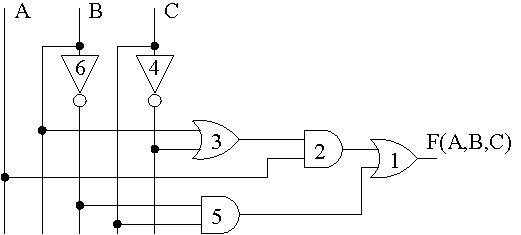
\includegraphics{advance}
\caption{The circuit diagram for $F(A,B,C)=A(B+C')+B'C$.}
\label{fig:representationsAdvance}
\end{figure}

During the parsing process, it is critically important to keep track of which 
parts of the expressions have been realized and which have not.  To 
do this, add lines under each of the subexpressions as they are created.
After correctly parsing the expression, each variable should have a little
line underneath it.  This parsing-management can be a dizzying process 
jumping between different levels of the parsing process to resume 
parsing pieces of the expression left unrealized.

\subsection{Symbolic to Symbolic}
The laws of ``regular" algebra are used to discover relationships
between expressions, and to manipulate expressions into more convenient forms.  
Boolean Algebra has a set of laws which can be employed to manipulate 
symbolic expressions.  The nine laws of Boolean Algebra are listed in 
Table~\ref{table:representationsLaws}.

\begin{table}
\begin{center}
\begin{tabular}[ht]{|c|c|c|}\hline
Law	&	Primary &	Dual	\\ \hline
1.	&	x+0=x	&	x*1=x	\\ \hline
2.	&	x+1=1	&	x*0=0	\\ \hline
3.	&	x+x=x	&	x*x=x	\\ \hline
4.	&	x''=x	&	     	\\ \hline
5.	&	x+x'=1		& x*x'=0	\\ \hline
6.	&	x+y=y+x		& x*y=y*x\\ \hline
7.	&	x+(y+z)=(x+y)+z	& x*(y*z)=(x*y)*z \\ \hline
8.	&	x*(y+z)=x*y+x*z	& x+(y*z)=(x+y)*(x+z)  \\ \hline
9.	&	(x+y)'=x'*y'  	& (x*y)'=x'+y' \\ \hline
\end{tabular}
\caption{The laws of Boolean Algebra using the Boolean variables $x,y,x$.}
\label{table:representationsLaws}
\end{center}
\end{table}

Notice that all laws (except Number 4) have a dual.  A dual of a 
symbolic expression is formed by swapping all ANDs and ORs and all 0s 
and 1s.  Boolean Algebra expresses the 
\textit{duality principle}: \index{duality principle}
If a statement $S$ is true, then the dual of $S$ is 
also true. Later, it will be convenient to identify which law is used
to manipulate a symbolic expression.  In these cases, write
down the law's number followed by D if it is a dual.  For example, if 
the property $x*x=x$ is used to manipulate a symbolic expression, then
indicate that Law 3D was used to manipulate the symbolic expression.

The laws in Table~\ref{table:representationsLaws} can be verified as true
by plugging in every possible combination of bits and checking if the two sides
of the equation are equal.  For example, to check Law 3D, set $x=0$, 
yielding $0*0=0$ which is true, and then set $x=1$ and verify that $1*1=1$.

The laws of Boolean Algebra can be used to prove two symbolic expressions are 
equal.  This proof is performed by manipulating one of the expressions until it
exactly equals the other side.  For example, to prove that $A + A'B' = A + B'$,
transform the more complex expression into the simpler
expression.  In the example, $A+A'B'$ is the more complex expression and $A+B'$
is the simpler expression.  At each step of the transformation 
provide the law used to yield the next step.

\begin{tabular}[ht]{ll}
$A + A'B' =$		& Law 8D \\
$(A+A')*(A+B')=$	& Law 5 \\
$1*(A+B')=$ 		& Law 1D \\
$A+B'$ \\
\end{tabular}

Working on these derivations is a little like solving a maze or playing
a good game of chess.  Both require a player to ``look ahead" and see what the 
implications of a decision will be.  Not looking far enough ahead may
result in arriving at one of the preceding steps.  For example, consider what 
happened in the following loopy-derivation of $A(A+B)=A$.  The correct 
derivation is shown on the right.

\begin{tabular}[ht]{ll|ll}
Loopy		&		& Correct	&		\\ \hline
$A(A+B)=$ 	& Law 8	& $A(A+B)=$ & Law 8	\\ 
$AA + AB=$ 	& Law 3D	& $A*A+A*B=$& Law 3	\\ 
$A+AB=$	& Law 8D	& $A+A*B$ 	& Law 1D	\\ 
$(A+A)(A+B)=$& Law 3	& $A*1+A*B$	& Law 8	\\ 
$A(A+B)$	& huh?	& $A(1+B)$	& Law 2	\\
		&		& $A(1)$	& Law 1D	\\
		&		& $A$		& \\
\end{tabular}

The \textit{expansion trick} can be used to show that two expressions are 
equal to one another.
\index{trick!expansion}  The first step in the expansion trick is
to remove all the parenthesis using Law 8 and reduce the expression
to a set of product terms ORed together. The second step in the 
expansion trick is to add the ``missing" variables to each product 
in the expression.  This second step is illustrated in the following
derivation.

\textbf{Show:} $A'B'C' + B'C + ABC = A'B' + AC$

\textbf{Derivation:} 

$\begin{array}[ht]{ll}
A'B'C' + B'C + ABC =		& \text{Law 1D} \\
A'B'C' + 1B'C + ABC = 		& \text{Law 3} \\
A'B'C' + (A+A')B'C + ABC = 	& \text{Law 8} \\
A'B'C' + AB'C +A'B'C + ABC = 	& \text{Law 6} \\
A'B'C' + A'B'C +AB'C + ABC = 	& \text{Law 8} \\
A'B'(C' + C) +AC(B' + B) = 	& \text{Law 5} \\
A'B'1 +AC1 = 			& \text{Law 1D} \\
A'B' +AC = 				&  \\
\end{array}$

Since both expressions consist of product terms, Law 8 need not be applied.
 The second step of the expansion trick,
adding the missing variable occurs when $B'C$ is expanded 
into $A'B'C + AB'C$.  In this case, the $B'C$ product term is 
``missing" the $A$ variable.  It is included by first ANDing 1 
with $B'C$, then replacing 1 with $(A+A')$, and finally
distributing $B'C$.  

Finishing this formal derivation is 
straightforward, but requires some scratch work.  Start by 
expanding the right-hand side of the derivation $A'B' + AC$,
using the expansion trick, into $A'B'C' + AB'C +A'B'C + ABC$ 
on some scratch paper.  Now, 
write the second to last step of the scratch work derivation underneath 
the $A'B'C' + AB'C +A'B'C + ABC$ expression in the formal 
derivation.  Then, write the third to last step of the scratch 
work derivation as the next step of the formal derivation.
Continue until $A'B'+AC$ is written as the last step in
the formal derivation.  This idea is similar to a common maze-solving 
strategy, work at both ends of the maze and try to meet 
in the middle. 

The expansion trick runs into problems when there are a large
number of terms in parenthesis.  With a large number
of terms in parenthesis, the distribution process becomes tedious
and error prone. The following derivation utilizes Laws
4 and 9 to avoid this problem.

\textbf{Show:} $(A+B)(A'+B)(B+C) = B$

\textbf{Derivation:}

$\begin{array}[ht]{ll}
(A+B)(A'+B)(B+C) = 			& \text{Law 4} \\
\left[ (A+B)(A'+B)(B+C) \right] '' =& \text{Law 9D} \\
\left[ (A+B)'+(A'+B)'+(B+C)' \right]' = & \text{Law 9} \\
\left[ A'B'+AB'+B'C' \right]' = 	& \text{Law 8} \\
\left[ B'(A'+A)+B'C' \right]' = 	& \text{Law 5} \\
\left[ [B'1+ B'C' \right]' = 		& \text{Law 1D} \\
\left[ B'(1+C') \right]' = 		& \text{Law 2} \\
\left[ B'1 \right]' = 			& \text{Law 1} \\
\left[ B' \right]' = 			& \text{Law 4} \\
B  &  
\end{array}$

The first step in the derivation, double negating the expression, establishes 
the conditions for the application of Law 9D. One of the negations is
pulled into the bracketed expression converting the product into 
the OR of each product term, negated.  As shown, Law 9 can be applied
to an expression with more than two terms.  In the next step, Law 9 is 
applied to each term in parenthesis.  What remains is a set of product 
terms inside the brackets.  Over the next five steps this product term 
is simplified.  In the final step, the second negation introduced 
back in the first step of the proof is combined with the $B'$ 
inside the brackets, yielding the desired result.

\subsection{Truth Table to Symbolic}
\label{sec:TTtoSymb}

The most technical transformation in the design process is transforming 
a truth table to symbolic expression.  The idea behind this conversion is 
captured by the following analogy.  Imagine eight members of the college 
cheer squad, each have a number between $0 \ldots 7$ pinned to his/her
uniform, are gathered together.  Whenever members of the squad hears
the number pinned to their uniform they give a cheer.  If a member hears
any other number, they do nothing, even if someone else is cheering like crazy.

In order to get a cheer whenever 1, 4, 6, or 7 was announced 
over the public address system, which members of the squad should be
selected?  Clearly, four members of the squad would be selected, the member
with number 1, the member with number 4, the member with number 6,
and the member with number 7.

The squad members in this analogy are circuit elements called 
\textit{minterms}. \index{minterm!definition} A minterm for a function 
is a Boolean expression evaluating to logic 1 for a single 
combination of the inputs and evaluates to logic 0 for every 
other input.  A cheering squad member corresponds to a minterm with 
an output of 1.  The number pinned to each squad member corresponds
to the binary input which causes the minterm to output 1.  In order 
to build a symbolic expression for a truth table, first select the
minterms corresponding to the inputs where the function equals 1.  
Next, OR together these minterms and label the output of
the OR gate with the function.  In the cheer squad analogy, the ability of
sound from any member of the cheer squad to be heard corresponds
to the OR gates.  

\paragraph{Minterms}
Up till now minterms have been abstract entities, albeit with
well-defined properties.  To change that, consider all
the minterms for a function  with three input variables 
$A,B,C$.  Since $F$ has eight different inputs, it will have eight 
minterms.  Next, build the minterm that ``recognizes" the input $A=B=C=1$.  
This task is accomplished by creating an expression which outputs 1 only when 
$A=B=C=1$.  In this case, the minterm is $ABC$ because it equals 
1 when all the inputs are 1, and for any other input, a 0.
This minterm is denoted $m_7$, the lowercase $m$ signifies that 
this is a minterm and the 7 denotes the decimal representation 
of the input which causes this minterm to equal 1.  

The minterm
for the input $A=0, B=1, C=0$, $m_2$, is $A'BC'$.  Negating the
$A$ and $C$ variables allows a 0 input value for these variables to 
be inverted to 1 before being ANDed.  

In order to make generating 
the remaining six minterms easier, formalize the observation 
just made and call it the \textit{minterm trick}.  
\index{trick!minterm} \label{page:MinTrick}
A minterm for a particular input needs to include all the variables.
If a variable's value is equal to 0, the variable should be negated in 
the AND expression, if its value is 1, it appears as itself in the
AND expression. The table below shows all the minterms for three 
variables A,B,C.

\begin{tabular}{c|c|c||c|c}
A & B & C & minterm & symbol	\\ \hline
0 & 0 & 0 & A'B'C'  & $m_0$	\\ \hline
0 & 0 & 1 & A'B'C   & $m_1$	\\ \hline
0 & 1 & 0 & A'BC'   & $m_2$	\\ \hline
0 & 1 & 1 & A'BC    & $m_3$	\\ \hline
1 & 0 & 0 & AB'C'   & $m_4$	\\ \hline
1 & 0 & 1 & AB'C    & $m_5$	\\ \hline
1 & 1 & 0 & ABC'    & $m_6$	\\ \hline
1 & 1 & 1 & ABC     & $m_7$	\\ 
\end{tabular}

A minterm is said to ``recognizes its input" when that input
causes the minterm to evaluate to 1.  Thus, minterm $m_3$ recognizes
the input $(A,B,C)=(0,1,1)$ and ignores all other inputs.  In order 
to construct the symbolic expression for a truth table, OR together 
the minterms for which the function equals 1. Thus, when any one of 
the minterms recognizes its input, one of the inputs to the OR gate 
will equal 1 causing the output of the OR gate to become 1.  Note, 
that at most one of the OR gates inputs will equal 1, since only one 
of the minterms will recognize its input.  If none of the minterms 
recognizes the input, all the inputs of the OR gate will equal 0, 
causing the output of the OR gate to equal 0.  To better understand
these concepts, consider the function $F(A,B,C)$ defined below.

\begin{tabular}{c|c|c||c|c|c}
A & B & C & F(A,B,C)	& minterm & symbol	\\ \hline
0 & 0 & 0 & 0		& A'B'C'  & $m_0$	\\ \hline
0 & 0 & 1 & 1		& A'B'C   & $m_1$	\\ \hline
0 & 1 & 0 & 1		& A'BC'   & $m_2$	\\ \hline
0 & 1 & 1 & 1		& A'BC    & $m_3$	\\ \hline
1 & 0 & 0 & 1		& AB'C'   & $m_4$	\\ \hline
1 & 0 & 1 & 0		& AB'C    & $m_5$	\\ \hline
1 & 1 & 0 & 0		& ABC'    & $m_6$	\\ \hline
1 & 1 & 1 & 1		& ABC     & $m_7$	\\ 
\end{tabular}
\\ \\
There are five inputs for which $F(A,B,C)$ equals 1, so the symbolic
expression for $F$ will include the five minterms from the rows where
$F$ equals 1.  Hence, 
$$F(A,B,C) =  A'B'C + A'BC' + A'BC + AB'C' + ABC$$
Now, examine what happens to $F$ for the input $(A,B,C)=(0,0,1)$.  
The minterm $m_1=A'B'C$ evaluates to 1 while all the other minterms 
evaluate to 0.  Since the OR function evaluates to 1 when any of 
the inputs are equal 1, $F$ equals to 1. Hence, $F(0,0,1)=1$ as
expected.  When $(A,B,C)=(1,1,0)$ is applied, all the
minterms in the symbolic expression for $F$ evaluate to 0 because
none of them recognize this input.  Thus, $F(1,1,0)=0$ as expected.

When a function is constructed by ORing together minterms, it is
said to be in \textit{canonical sum of products} 
\index{SOP!canonical} form or canonical SOP form.  A symbolic
expression is said to be in SOP form when it consists
exclusively of a collection of product terms ORed together.  
The term sum/product is used to refer to the operators OR/AND 
respectively because these are what the operators look like in 
normal arithmetic. The term canonical is used because this 
symbolic form is the most elementary form possible to describe 
the function.

The canonical SOP representation for $F$ defined above can be 
abbreviated as $F(A,B,C) = \sum m(1,2,3,4,7)$  where the $\sum$
symbol denotes the ORing together of minterms 1,2,3,4 and 7.
In general, $\sum m(list)$ describes the inputs for which the
function equals 1.  When asked for a canonical SOP expression
in the homework, write either the symbolic expression
out, or use this abbreviated form.

Engineers are always striving to minimize the cost of their solutions.
Towards this end, a second way to transform a truth table into a 
symbolic expression is introduced.  It replaces the minterms with 
a different kind of building block, the maxterm.

\paragraph{Maxterms}
\index{maxterm!definition}
A \textit{maxterm} for a function is a symbolic expression evaluating
to 0 for a single combination of the inputs and evaluates to 1 for 
every other input.  Before constructing symbolic expressions for
a truth table, it is necessary to examine the structure of maxterms.

Since the function $F(A,B,C)$ has three inputs, it will have eight 
maxterms.  Start by creating the maxterm for the input $(A,B,C)=(0,0,0)$.
Many different expressions can be derived which equal 0 only for
this input, but the simplest is $A+B+C$.  This maxterm is
abbreviated $M_0$, the uppercase $M$ signifying a maxterm 
and the 0 denoting the decimal representation of the input which 
causes this maxterm to equal 0.  The \textit{maxterm trick} 
\index{trick!maxterm} is used to simplify the process of creating
maxterms.  

A maxterm for a particular input needs to include all the variables.
If a variable's value is equal to 1, the variable should be negated 
in the OR expression; if its value is 0, the expression appears as itself in the
OR expression. The table below lists all the maxterms for the three 
variables $A,B,C$.

\begin{tabular}{c|c|c||c|c}
A & B & C & maxterm   & symbol \\ \hline
0 & 0 & 0 & A+B+C     & $M_0$   \\ \hline
0 & 0 & 1 & A+B+C'    & $M_1$   \\ \hline
0 & 1 & 0 & A+B'+C    & $M_2$   \\ \hline
0 & 1 & 1 & A+B'+C'   & $M_3$   \\ \hline
1 & 0 & 0 & A'+B+C    & $M_4$   \\ \hline
1 & 0 & 1 & A'+B+C'   & $M_5$   \\ \hline
1 & 1 & 0 & A'+B'+C   & $M_6$   \\ \hline
1 & 1 & 1 & A'+B'+C'  & $M_7$   \\ 
\end{tabular}


In order to construct the symbolic expression for a truth table, 
AND together the maxterms for which the function equals 0. Thus, 
when any one of the maxterms recognizes its input, one of the 
inputs to the AND gate will equal 0, causing the output of the 
AND gate to go to 1.  Note, that at most one of the AND gate's 
inputs will equal 0, since only one of the maxterms will recognize 
the input.  If none of the maxterms recognizes the input, all the 
inputs of the AND gate equal 1, causing the output of the 
AND gate to equal 1.  These ideas are applied to 
the function $F(A,B,C)$ below.

\begin{tabular}{c|c|c||c|c|c}
A & B & C & F(A,B,C) & maxterm   & symbol \\ \hline
0 & 0 & 0 & 0        & A+B+C     & $M_0$   \\ \hline
0 & 0 & 1 & 1        & A+B+C'    & $M_1$   \\ \hline
0 & 1 & 0 & 1        & A+B'+C    & $M_2$   \\ \hline
0 & 1 & 1 & 1        & A+B'+C'   & $M_3$   \\ \hline
1 & 0 & 0 & 1        & A'+B+C    & $M_4$   \\ \hline
1 & 0 & 1 & 0        & A'+B+C'   & $M_5$   \\ \hline
1 & 1 & 0 & 0        & A'+B'+C   & $M_6$   \\ \hline
1 & 1 & 1 & 1        & A'+B'+C'  & $M_7$   \\ 
\end{tabular}
\\ \\
There are three inputs of $F(A,B,C)$ equal to 0, so the symbolic
expression for $F$ includes the three maxterms from the rows where
$F$ equals 0.  Hence, 

$$F(A,B,C) =  (A+B+C)(A'+B+C')(A'+B'+C)$$

What happens when the input $(A,B,C)=(1,0,1)$ is applied?  
The maxterm $M_5=(A'+B+C')$ evaluates to 0 while all the other maxterms 
evaluate to 1.  Since the AND function evaluates to 0 when any of 
the inputs are equal 0, $F$ equals to 0. Hence, $F(1,0,1)=0$ as
expected.  When $(A,B,C)=(1,1,1)$ is applied, all the
maxterms in the symbolic expression for $F$ evaluate to 1 because
none of them recognize this input.  Thus $F(1,1,1)=1$ as expected.

\index{POS!canonical}
This representation of $F$ is called its \textit{canonical product of sums} 
form or canonical POS form, because $F$ is represented in its most
elementary form as the AND (product) of a collection of OR (sum) terms.  
The canonical POS representation in the example can be abbreviated by 
the expression $F(A,B,C) = \prod M(0,5,6)$  where the $\prod$
symbol denotes the AND, the $M$ symbol stands for maxterm, and the 
numbers in the list are the inputs for which $F(A,B,C)$ equals 0.

Notice, the functions in the two minterm and maxterm examples are the 
same.  This was done to illustrate two points.  First, the inputs 
present in the minterm list are those that do not appear in the maxterm 
list.  In other words, $F(A,B,C) = \sum m(1,2,3,4,7) = \prod M (0,5,6)$.  
This should make sense. The minterm list denotes those inputs for 
which the function equals 1.  If the function does not equal 1 for 
a particular input, this input is not in the minterm list, and then the 
function must equal 0 for this input, hence this input will appear 
in the maxterm list.

The second reason for using the same function is to illustrate
how different realizations of the same function have different costs.
A solution requiring fewer gates
will cost less.  The following table summarizes the number of gates 
required in the SOP and POS realization of $F(A,B,C)$.
\\ \\
\begin{tabular}[ht]{l|c|c}
		    & SOP 	& POS	\\ \hline
 number of NOTs & 3	& 3	\\ \hline
 number of ANDs & 5	& 1	\\ \hline
 number of ORs  & 1	& 3	\\ 
\end{tabular}
\\ \\
Assuming that AND gates and OR gates have the same cost then the POS 
solution costs less.  Thus a good engineer would recommend a 
canonical POS realization over a canonical SOP realization.

While, the transformation from a truth table to a symbolic expression
may be the most technically challenging, it is certainly not the
most difficult.  This title belongs to the transformation of a word
statement into a truth table.  The difficulty of this transformation
has its origin in the puffy cloud outline of a word statement shown in
Figures \ref{fig:representtationsDesign} \ref{fig:representationsForms}. Words can be ambiguous and 
the ability of authors to convey precisely what the digital system
needs to accomplish depends on their skill with the English language.

\subsection{Word Statement to Truth Table}
There is no algorithmic approach guaranteed to transform a word statement 
into a truth table.  That said, the following list outlines essential
information to obtain from the word statement in order to
have any hope of transforming it into a truth table.

\begin{description}
\item [Step 1] Understand the number and meaning of the
inputs and the outputs of the digital system.  The meaning of inputs
will vary from system to system.  Typically, the inputs are broken into
collections of bits.  Each collection will have its own meaning attached
to it.

\item [Step 2] Write down an empty truth table.  If
the digital system has $N$ bits of input, then the truth table
has $2^N$ rows.  

\item [Step 3] Use the word statement to determine the output for 
each input, one row at a time.  This requires understanding what the inputs 
and outputs mean and then determining the relationship between each
input and output pair.
\end{description}

The following example shows how to apply these steps to a word statement.

\begin{quote}
Determine the truth table for 
a function with two bits of input and one bit of output.  The
output equals 1 when all the inputs are equal to 1.
\end{quote}

The 3-step process for transforming a word statement into a 
truth table are shown below.

\begin{description}
\item [Step 1] The function has two bits of input and one bit of output.  
Since the inputs and output were not given names, use the default labels
$A,B$ for the inputs and $F$ for the output.

\item [Step 2] The truth table for a 2-variable function has four 
rows.

	\begin{tabular}{c|c||c}
	A & B & F \\ \hline \hline
	0 & 0 &   \\ \hline
	0 & 1 &   \\ \hline
	1 & 0 &   \\ \hline
	1 & 1 &   \\
	\end{tabular}

\item [Step 3] The only row of the truth table where $A$ and $B$ both
equal to 1 is the last row; set this row's output equal to 1.  
All the other rows of the table have $F=0$ because they have
at least one input which equals 0.

	\begin{tabular}{c|c||c}
	A & B & F \\ \hline \hline
	0 & 0 & 0  \\ \hline
	0 & 1 & 0  \\ \hline
	1 & 0 & 0  \\ \hline
	1 & 1 & 1  \\
	\end{tabular}
\end{description}

This should be recognizable as the AND function.  In the
AND example, each of the bits was a distinct input by itself.  
Sometimes, the inputs work together to form some larger unit of
information, like a binary number.  This is the case in the next
example.

\begin{quote}
Determine the truth table for a function with three bits of input and
one bit of output.  The output of the function should equal 1 when
the 3-bit binary input represents a binary number greater than 4.
\end{quote}

\begin{description}
\item [Step 1] The function has three bits of input and one bit of output.  
Since the inputs and outputs were not given names, use the default labels
$a_2,a_1,a_0$ for the inputs and $F$ for the output.  The input
variables are given subscripts because they are working together to 
form a 3-bit binary number.  The binary number is referred to as
$A$ and its individual bits as $a_2$, $a_1$, and $a_0$.  Hence,
when $(a_2,a_1,a_0) = (1,0,1)$ then $A=5$.

\item [Step 2] Many 3-variable truth tables have been shown in this
chapter.  The notable point in this example is that the output is 
abbreviated as $F(A)$ to save space.

$\begin{array}[ht]{l|l|l||l}
a_2 & a_1 & a_0 & F(A)		\\ \hline
0   & 0   & 0   &		\\ \hline
0   & 0   & 1   &		\\ \hline
0   & 1   & 0   &		\\ \hline
0   & 1   & 1   &		\\ \hline
1   & 0   & 0   &		\\ \hline
1   & 0   & 1   &		\\ \hline
1   & 1   & 0   &		\\ \hline
1   & 1   & 1   &		\\ 
\end{array}$

\item [Step 3] The output of the function equals 0 for all inputs
less than or equal to $(a_2,a_1,a_0) = (1,0,0)$ and equals 1 for 
inputs greater or equal to $(a_2,a_1,a_0) = (1,0,1)$.  This yields
the following truth table.

$\begin{array}[ht]{l|l|l||l}
a_2 & a_1 & a_0 & F(A)		\\ \hline
0   & 0   & 0   &	0	\\ \hline
0   & 0   & 1   &	0	\\ \hline
0   & 1   & 0   &	0	\\ \hline
0   & 1   & 1   &	0	\\ \hline
1   & 0   & 0   &	0	\\ \hline
1   & 0   & 1   &	1	\\ \hline
1   & 1   & 0   &	1	\\ \hline
1   & 1   & 1   &	1	\\ 
\end{array}$

\end{description}

In the third and final example, there are two twists.  The truth
table will describe a function with four variables and the function
has three bits of output.  For the sake of brevity, the second and the 
third steps of the transformation process are combined.

\begin{quote}
Determine the truth table for a digital system having two, 2-bit 
inputs $A=a_1 a_0$ and $B=b_1 b_0$. Each 2-bit input represents a 
2-bit binary number.  The function has three bits of output called
$G$, $L$, and $E$, which stand for greater, less, and equal, respectively.
$E$ equals 1 when $A=B$, $G=1$ when $A>B$, and $L=1$ when $A<B$.
\end{quote}

\begin{description}
\item [Step 1] The function has four bits of input and three bits of output.
The names of these variables are clear from the word statement.

\item[Step 2 \& 3]  The truth table for this function has 16 rows
because there are $2^4=16$ combinations of four bits 
(see page~\pageref{page:two-to-N}).
In order to better visualize the solution to the problem, the values of $A$ and
$B$ (derived from their values of $a_1,a_0$ and $b_1,b_0$) are included 
in the truth table.  

$$\begin{array}{c|c|c|c||c|c||c|c|c}
a_1 & a_0 & b_1 & b_0 & A & B & G & L & E \\ \hline
0 & 0 & 0 & 0 & 0 & 0 & 0 & 0 & 1  \\ \hline
0 & 0 & 0 & 1 & 0 & 1 & 0 & 1 & 0  \\ \hline
0 & 0 & 1 & 0 & 0 & 2 & 0 & 1 & 0  \\ \hline
0 & 0 & 1 & 1 & 0 & 3 & 0 & 1 & 0  \\ \hline
0 & 1 & 0 & 0 & 1 & 0 & 1 & 0 & 0  \\ \hline
0 & 1 & 0 & 1 & 1 & 1 & 0 & 0 & 1  \\ \hline
0 & 1 & 1 & 0 & 1 & 2 & 0 & 1 & 0  \\ \hline
0 & 1 & 1 & 1 & 1 & 3 & 0 & 1 & 0  \\ \hline
1 & 0 & 0 & 0 & 2 & 0 & 1 & 0 & 0  \\ \hline
1 & 0 & 0 & 1 & 2 & 1 & 1 & 0 & 0  \\ \hline
1 & 0 & 1 & 0 & 2 & 2 & 0 & 0 & 1  \\ \hline
1 & 0 & 1 & 1 & 2 & 3 & 0 & 1 & 0  \\ \hline
1 & 1 & 0 & 0 & 3 & 0 & 1 & 0 & 0  \\ \hline
1 & 1 & 0 & 1 & 3 & 1 & 1 & 0 & 0  \\ \hline
1 & 1 & 1 & 0 & 3 & 2 & 1 & 0 & 0  \\ \hline
1 & 1 & 1 & 1 & 3 & 3 & 0 & 0 & 1  \\ 
\end{array}$$
\end{description}

In order to transform this truth table into a symbolic expression, 
realize each of the three outputs are independent of the
others.  For example, to determine the symbolic expression for $G$,
cover-up the output columns corresponding to the $L$ and $E$ outputs
and implement $G$.  In order to realize $L$, just cover-up the 
columns associated with $G$ and $E$ and implement $L$ as if
the other two outputs did not exist.  This yields the following
three equations for the outputs.

$$\begin{array}{l}
G(a_1,a_0,b_1,b_0)=\sum m(4,8,9,12,13,14)	\\
L(a_1,a_0,b_1,b_0)=\sum m(1,2,3,6,7,11)	\\
E(a_1,a_0,b_1,b_0)=\sum m(0,5,10,15)	\\
\end{array}$$

Of course this leads to the question of how to build the circuit
diagram for this 4-input, 3-output function.  Students often
want to OR together the $G$, $L$, and $E$ outputs in order to have
a single output, but this is would be incorrect because the word 
statement asked for three separate outputs.  The correct way to build
the circuit diagram is to build each of the circuits separately, give
each its own output, and have them share the same inputs.  A rough
sketch of the circuit is shown in Figure~\ref{fig:representationsThreeOutputs}.

\begin{figure}[ht]
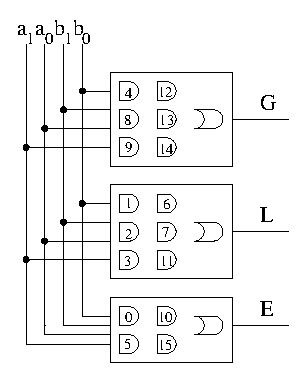
\includegraphics{ThreeOutputs}
\caption{The circuit diagram for a circuit which compares the 
magnitude of the two inputs $A=a_1 a_0$ and $B=b_1 b_0$.  Many of 
the internal details have been omitted.}
\label{fig:representationsThreeOutputs}
\end{figure}

Notice that the three output circuits share the same inputs, but otherwise
are independent of one another.  Sharing inputs allows each
circuit to coordinate its output with the other circuits.  When
each circuit does what it is supposed to do for that input, the
output looks like a unified whole even though it is generated from
three separate circuits.

\section{Timing Diagrams}
\index{timing!diagrams}
After a circuit has been realized in hardware, the logical
representation of 0s and 1s is replaced by physical voltages
representing these logic levels.  In order to observe the behavior
of a physical digital system, an engineer typically uses a
logic analyzer or oscilloscope.  The waveforms drawn by the logic
analyzer when applying inputs and examining the outputs is called
a \textit{timing diagram}.  A timing diagram is a graph of the logic value 
of a signal versus time.  Typically, several signals are combined on the
same timing diagram to save space and in order to clearly 
show the relationship between the signals.

It is imperative to check if the digital system implemented
behaves according to its specification. Hence, an understanding of
timing diagrams is essential.  With a small circuit it is reasonable
to apply every possible combination of inputs and examine the 
output of the circuit.  For example, Figure~\ref{fig:represenationsTime} shows
the timing diagram for $F(A,B,C) = A'B+AB'C$.

\begin{figure}[ht]
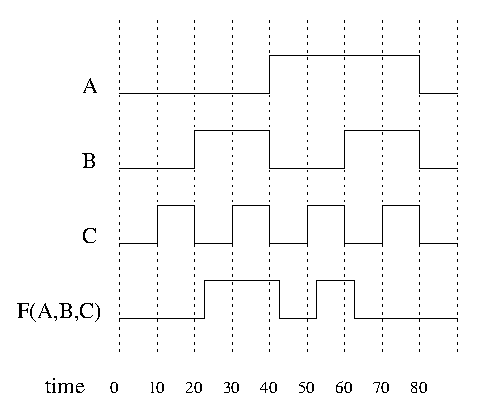
\includegraphics{time}
\caption{A timing diagram for $F(A,B,C) = A'B + AB'C$.}
\label{fig:represenationsTime}
\end{figure}

Observe that the time intervals are spaced 10 units apart.  For
now, the meaning of the units is unimportant.  Most likely, they would
be nanoseconds.  In practice, the timing behavior of a circuit
may be very important because circuits must not only have the 
correct output, but the circuit must meet strict timing constraints.

At time=5 the input $(A,B,C)=(0,0,0)$ and the output in response
to this input is 0.  At time=15 the input is $(0,0,1)$, and the
output due to this input is 0.  At time=75 the input is $(1,1,1)$
and the output is 0.  Every combination of the inputs has been 
applied to the circuit allowing the test engineer to verify the 
functional behavior of the circuit.

\subsection{Propagation Delay}
Notice that when the inputs change at time=20, the output $F$ 
transitions from 0 to 1 a little after time=20. This delay in the 
output transition is a manifestation of a real physical effect 
called \textit{propagation delay} \index{propagation delay}.  
\begin{quote}
Propagation delay is the time difference between the application of 
inputs and when the outputs becoming valid. 
\end{quote}
The physical basis of propagation delay is due to the finite amount 
of time required to charge or discharge a capacitor.  Propagation delay
is a limiting factor in processor speeds and has been know to cause
logical errors in circuit behavior.  It is so important that parts vendors
state the propagation delays of their circuits.  For example, 
consulting the technical documents for the Texas Instruments
74LS32, an OR gate, reveals four different values for propagation
delay: A typical, and a maximum value for both \Tphl and \Tplh.

\begin{tabular}{c|c|c}
         & TYPICAL & MAX  \\ \hline
\Tplh    & 10nS    & 15nS \\ 
\Tphl    & 14nS    & 22nS \\
\end{tabular}
\\ \\
\Tphl stands for the propagation delay to switch the output from
logic 1 to logic 0.  Likewise, \Tplh stands for the propagation delay 
to switch the output from 0 to 1. The TYPICAL and MAX columns 
give the tolerances the manufacture guarantees.  To simplify
analysis, the largest maximum delay can be used as a single value
for the propagation delay.  For example, it is safe to assume that
the outputs of a 74LS32 will switch in 22nS. 

%\subsection{Hazards}
%\section{VHSIC Hardware Description Language}
%\subsection{Entity and Architecture}
%\subsection{Concurrent Signal Assignment Statements}
